\documentclass[12pt]{article}
\usepackage[a5paper,margin=7mm,bottom=15mm]{geometry}
\usepackage{graphicx,color}
\usepackage{multicol}
\title{Tema 1 - Calcul numeric - an I ID}
\date{Due March 28, 2021 6:59 PM}
\author{Dinu Eugen Cosmin}

\begin{document}
\maketitle
\thispagestyle{empty}

% Proper formatting of paragraph with sloppypar
\begin{sloppypar}
Instructions

Se se rezolve urmatoarele exercitii. Rezolvarile se vor scrie intr-un fisier (se pot include si poze ale rezolvarilor problemelor pe hartie).

1. Sa se determine o solutie a ecuatiei $f(x)=0$ unde $f(x)=x^3-x^2-x+1$  folosind metoda lui Newton cu valorea initiala $x_0=-0.2$ si $epsilon=0.01$.

2. Sa se determine o solutie a ecuatiei $f(x)=0$ unde $f(x)=8x^3+x^2+8x-3$ folosind metoda secantei cu $0.0$ si $0.6$ valori initiale si $epsilon=0.01$.

3. Sa se determine o solutie a ecuatiei $f(x)=0$ unde $f(x)=x^3-4x+2$ folosind metoda bisectiei cu valorile initiale $a=0, b=1, epsilon=0.01$.

4. Se da functia de la exercitiul 3. Daca $x_1=1$, cat este $x_2$ din metoda lui Newton-Raphson?

5. Se da functia de la exercitiul 3. Daca $x_0=0$ si $x_1=1$, cat sunt $x_2$ si $x_3$ din metoda secantei?
\end{sloppypar}
\pagebreak

Rezolvări:\\

(1) $f(x)=x^3-x^2-x+1, f(x)=0, x=?$, prin metoda lui Newton-Raphson,
având $x_0=-0.2, \varepsilon=0.01$.
\begin{multicols}{2}
\scriptsize
\begin{verbatim}
# Cod octave:
f = @(x) x.^3-x.^2-x+1;
df = @(x) 3*x.^2-2*x-1;
epsilon = 0.01;
x_0 = -0.2;
x_1 = x_0 - (f(x_0) / df (x_0));

while epsilon < abs(f(x_1))
    # Urmatoarea estimare a solutiei
    x_1 = x_0 - (f(x_0) / df (x_0));
    print_graph(f, df, x_0, x_1, iter_count);
    x_0 = x_1;
endwhile
\end{verbatim}
\end{multicols}

\begin{figure}[htbp]
    \begin{center}
        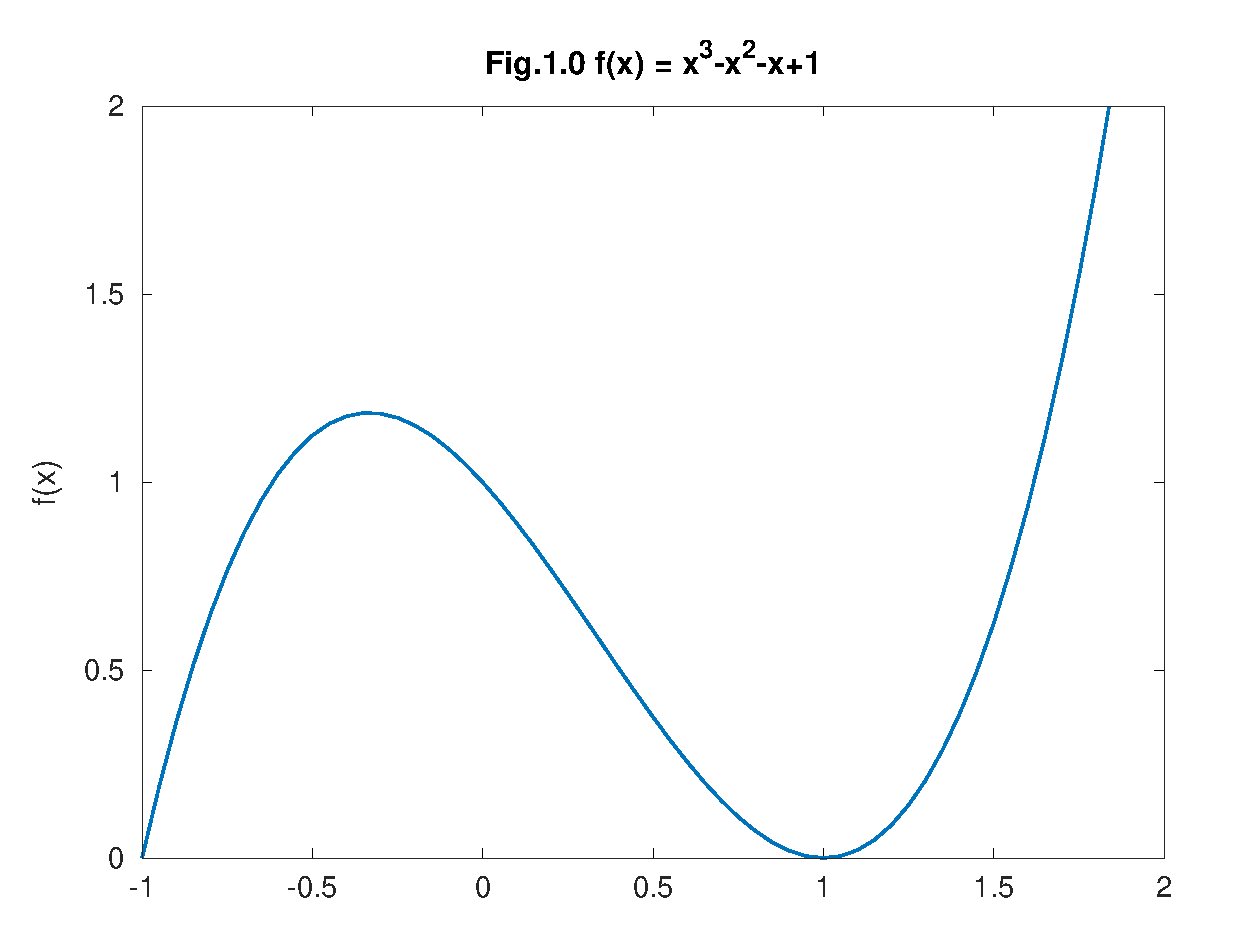
\includegraphics[height=90mm]{octave-fig/Fig.1.0.eps}
    \end{center}
\end{figure}

Sirul solutiilor aproximate este:\\
$X=\{2.200000,1.694737,1.387033,1.208029,1.108694,1.055712,1.0557\}$\\
$x_7=1.0557, f(x_7)=0.00638065, f(x_7) < \varepsilon$,\\
deci $solutia=x_7=1.0557$.

\begin{figure}[htbp]
    \begin{center}
        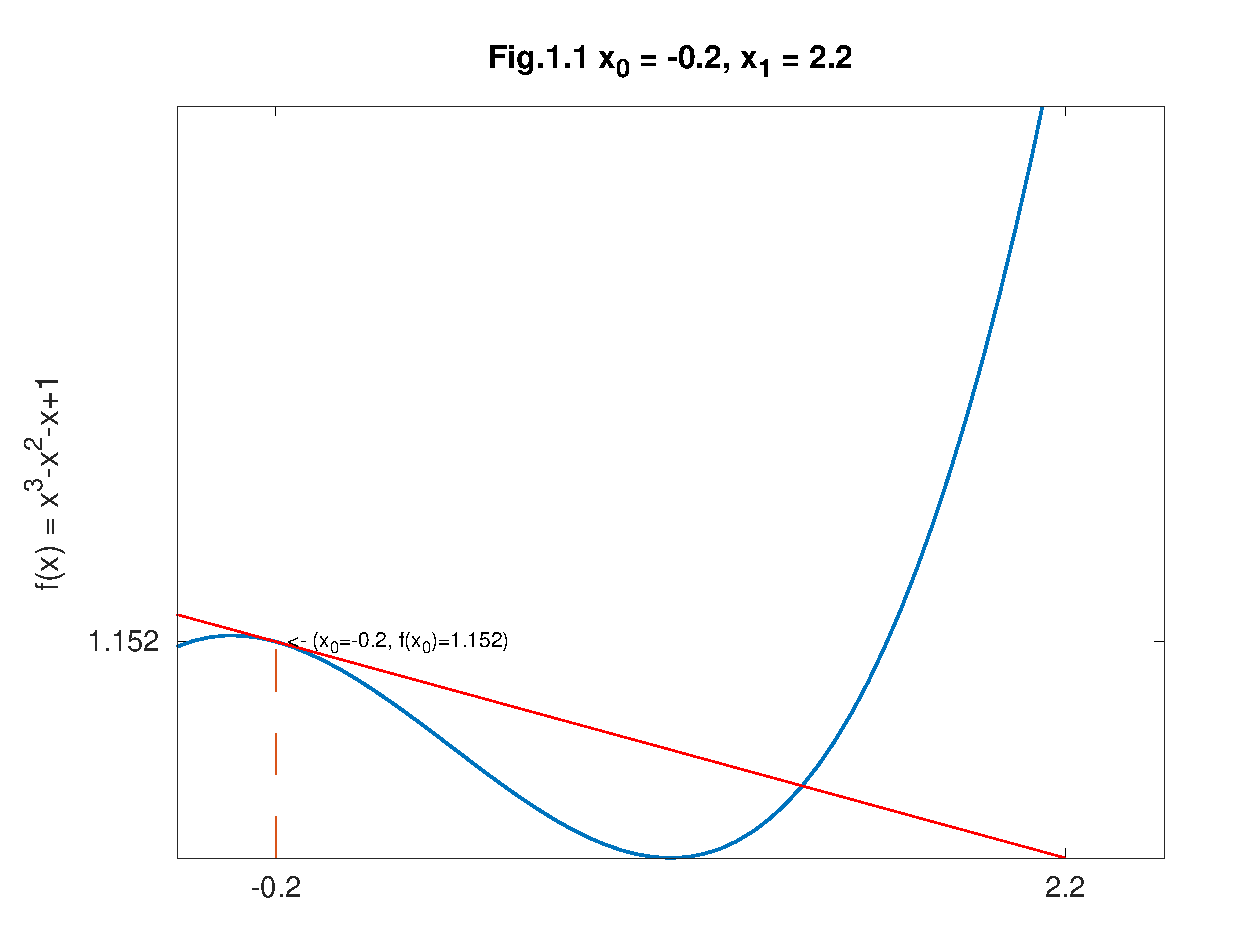
\includegraphics[height=90mm]{octave-fig/Fig.1.1.eps}
        \includegraphics[height=90mm]{octave-fig/Fig.1.2.eps}
    \end{center}
\end{figure}
\begin{figure}[htbp]
    \begin{center}
        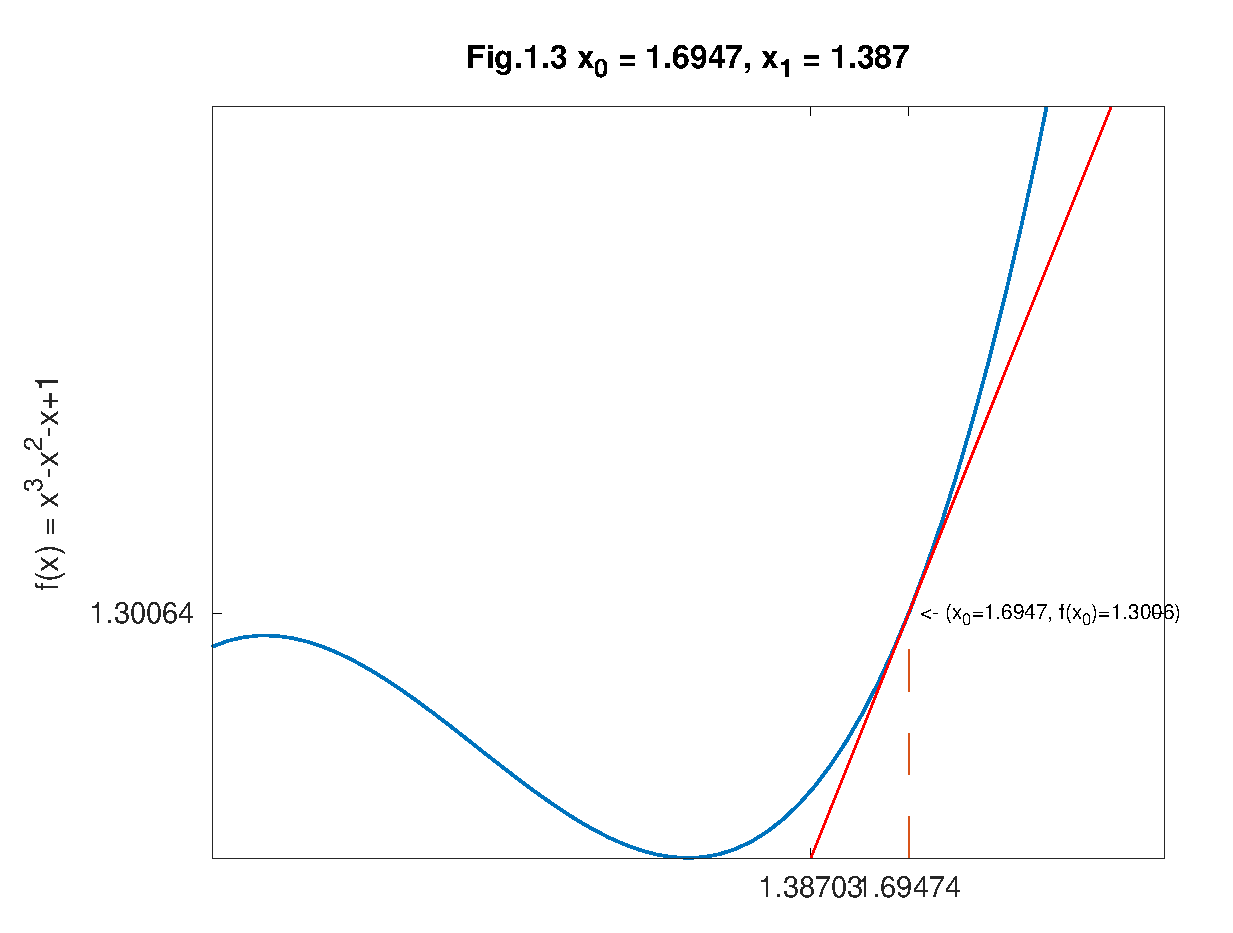
\includegraphics[height=90mm]{octave-fig/Fig.1.3.eps}
        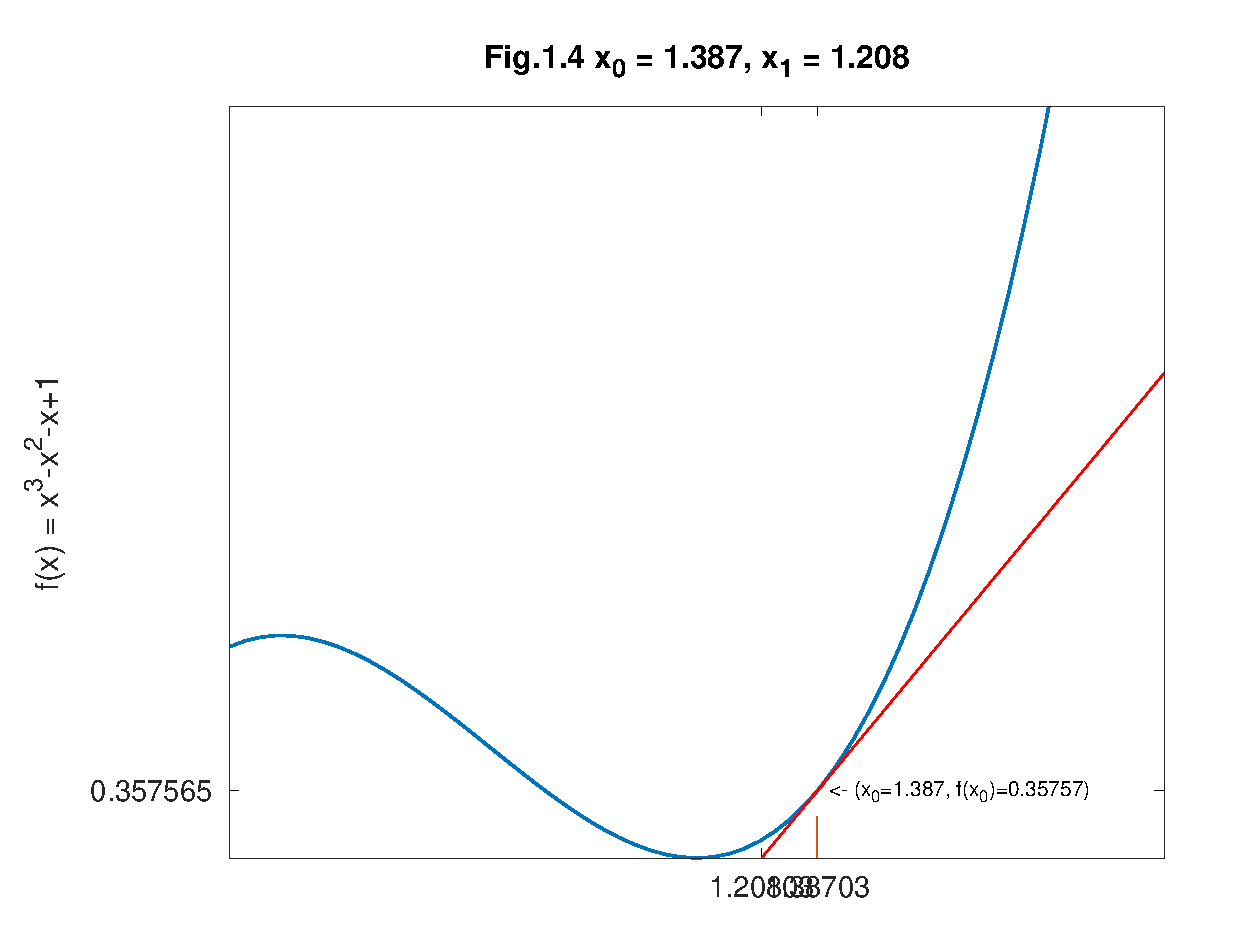
\includegraphics[height=90mm]{octave-fig/Fig.1.4.eps}
    \end{center}
\end{figure}
\begin{figure}[htbp]
    \begin{center}
        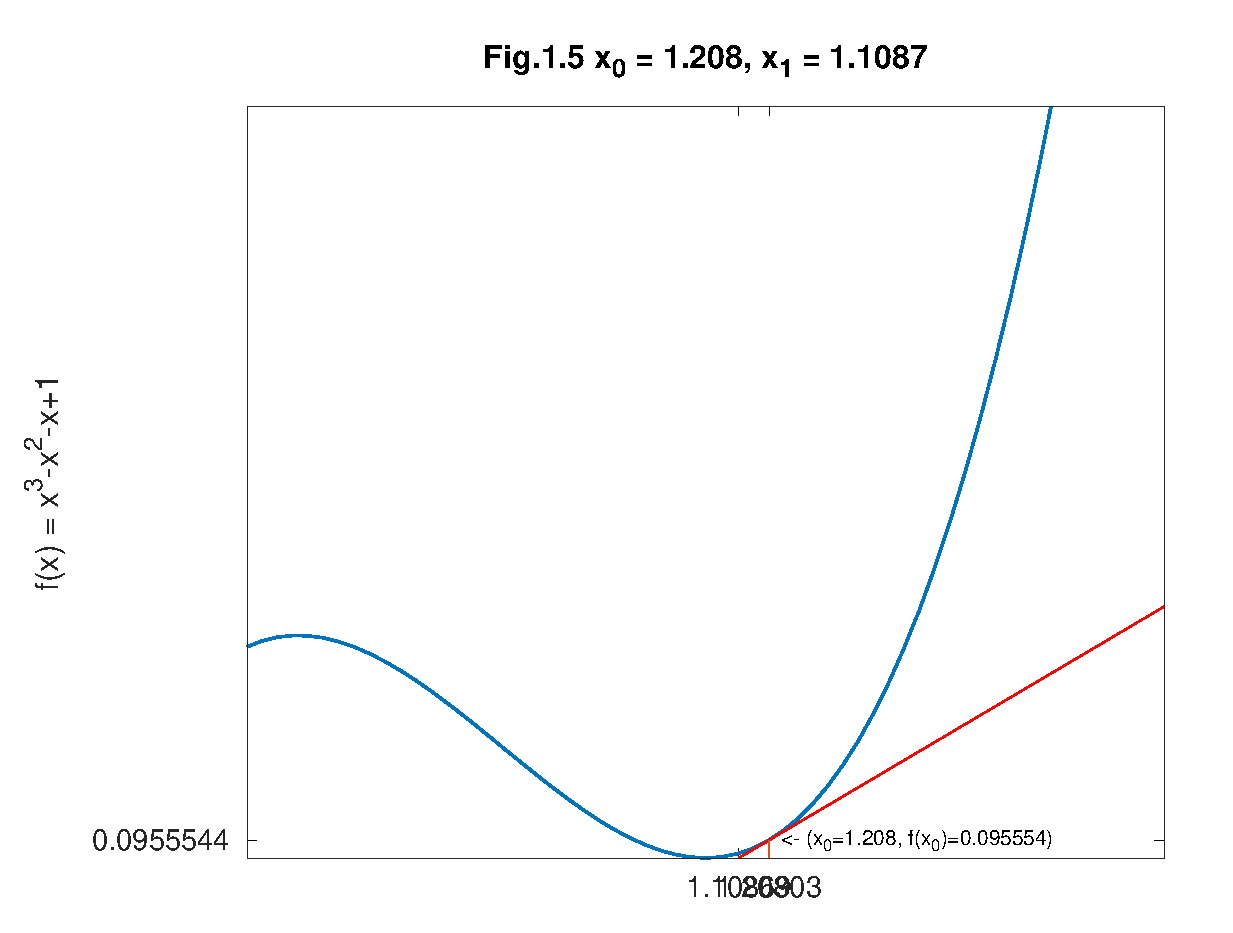
\includegraphics[height=90mm]{octave-fig/Fig.1.5.eps}
        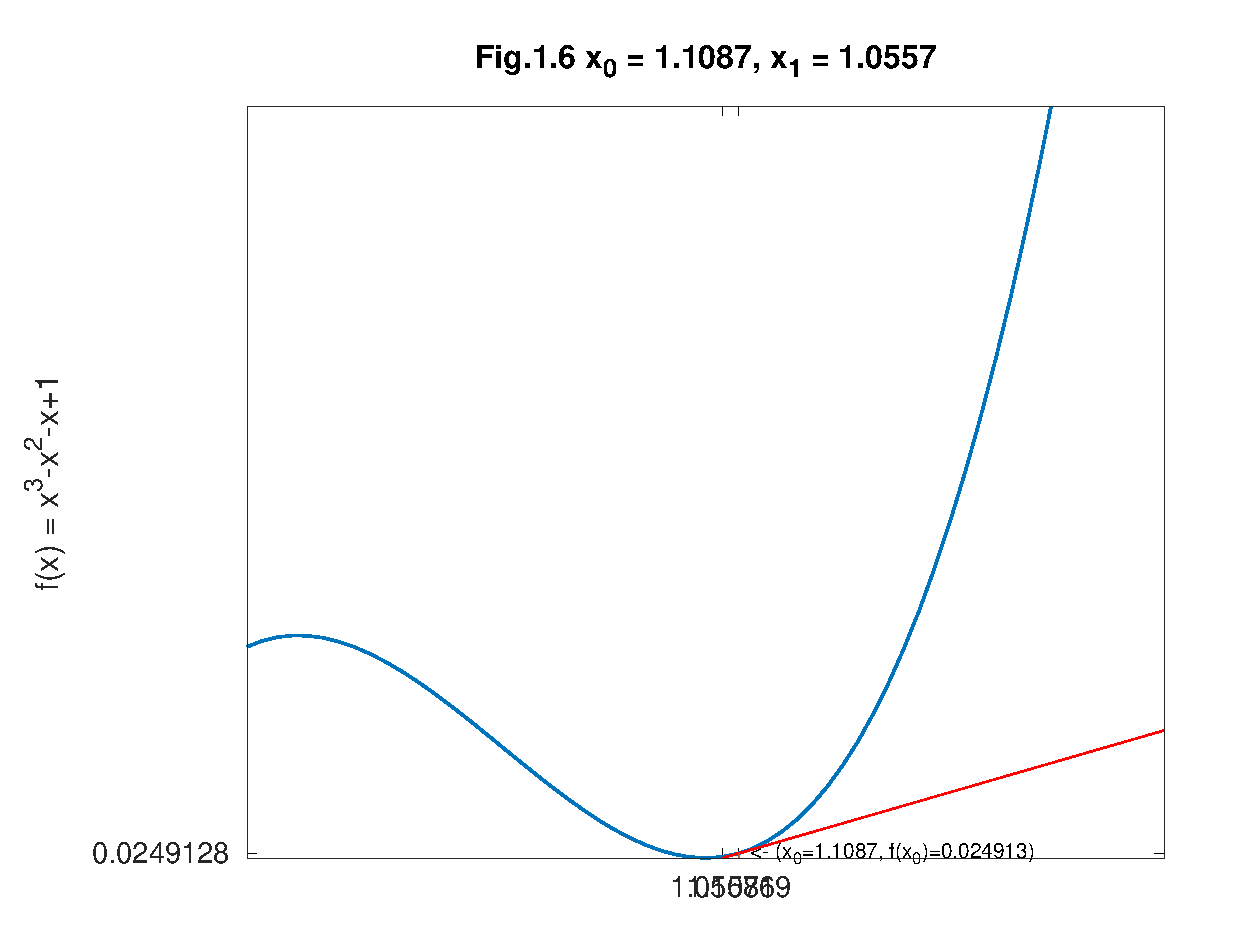
\includegraphics[height=90mm]{octave-fig/Fig.1.6.eps}
    \end{center}
\end{figure}
\begin{figure}[htbp]
    \begin{center}
        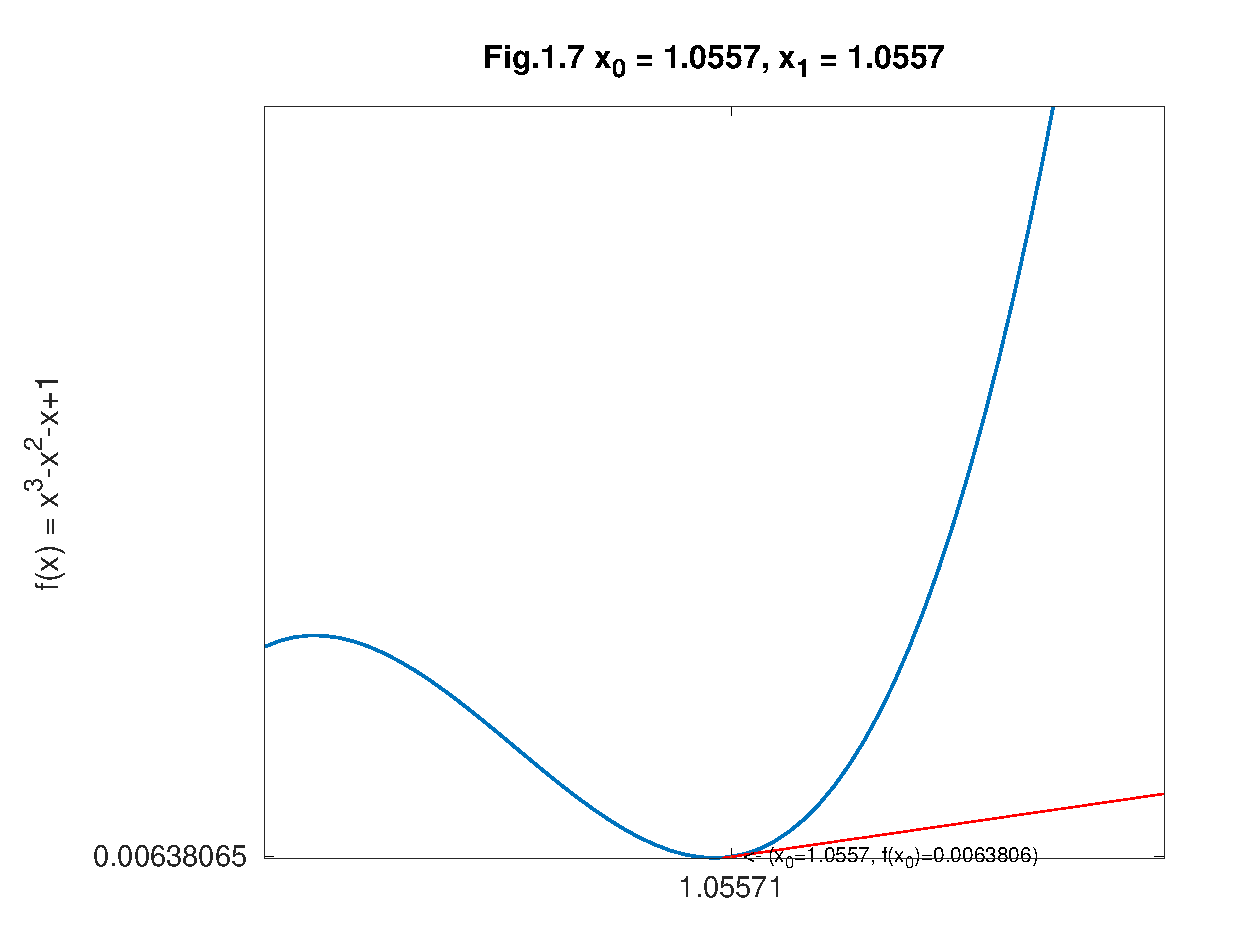
\includegraphics[height=90mm]{octave-fig/Fig.1.7.eps}
    \end{center}
\end{figure}
\newpage


(2) $f(x)=8x^3+x^2+8x-3, f(x)=0, x=?$, prin metoda secantei, având $0.0, 0.6$ valori initiale si $\varepsilon=0.01$.

\scriptsize
\begin{verbatim}
    # Cod octave:
    i = 1;
    i_max = 5;
    while abs(f(x_0)) > epsilon && i < i_max 
        x_1 = x_1 - (f(x_1)*(x_1-x_0))/(f(x_1)-f(x_0));
        print_graph(f, x_0, x_1, i);
        i ++;
    endwhile
\end{verbatim}

\begin{figure}[htbp]
    \begin{center}
        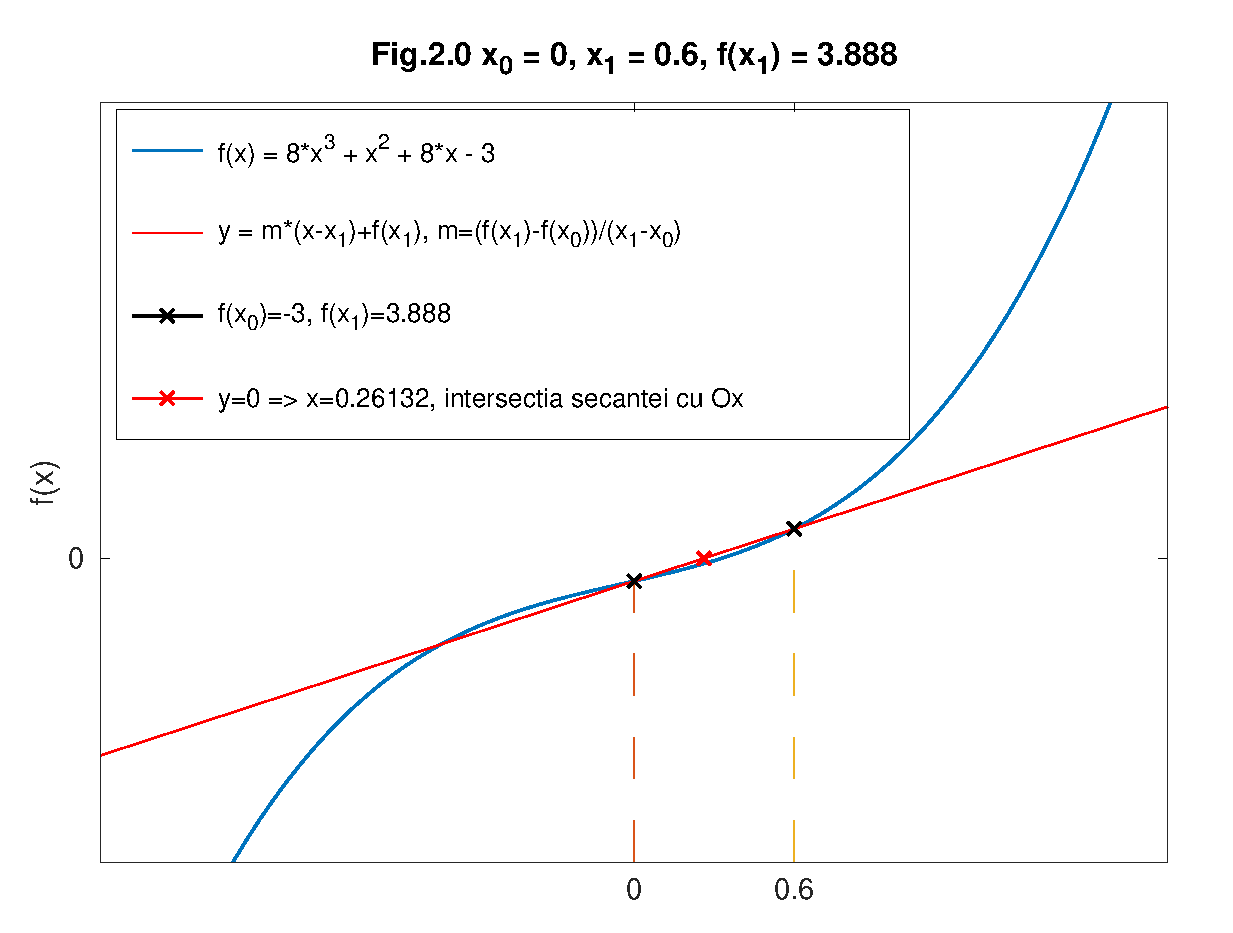
\includegraphics[height=90mm]{octave-fig/Fig.2.0.eps}
    \end{center}
\end{figure}
\normalsize
\begin{center}
\begin{tabular}{ c | c | c | c }
    i=1 & x_0=0.00 & x_1=0.261324 & f(x_1)=-0.698350 \\ \hline
    i=2 & x_0=0.00 & x_2=0.340613 & f(x_2)=0.157059 \\ \hline
    i=3 & x_0=0.00 & x_3=0.323668 & f(x_3)=-0.034631 \\ \hline
    i=4 & x_0=0.00 & x_4=0.327448 & f(x_4)=0.007685 \\
\end{tabular}
\end{center}
$f(x_4)=0.007685 < \varepsilon = 0.01$, \\
deci $solutia = 0.007685$.
\begin{figure}[htbp]
    \begin{center}
        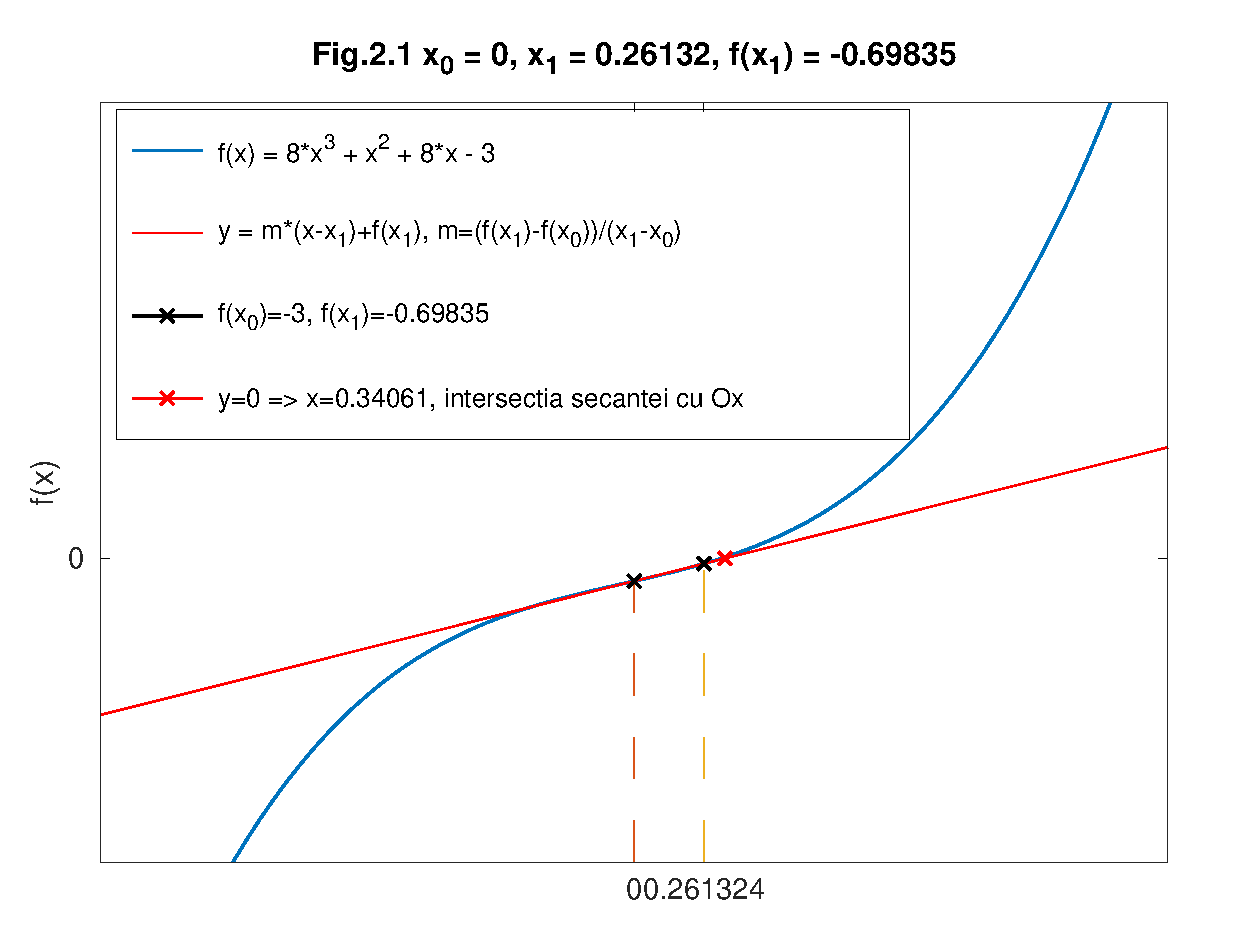
\includegraphics[height=90mm]{octave-fig/Fig.2.1.eps}
        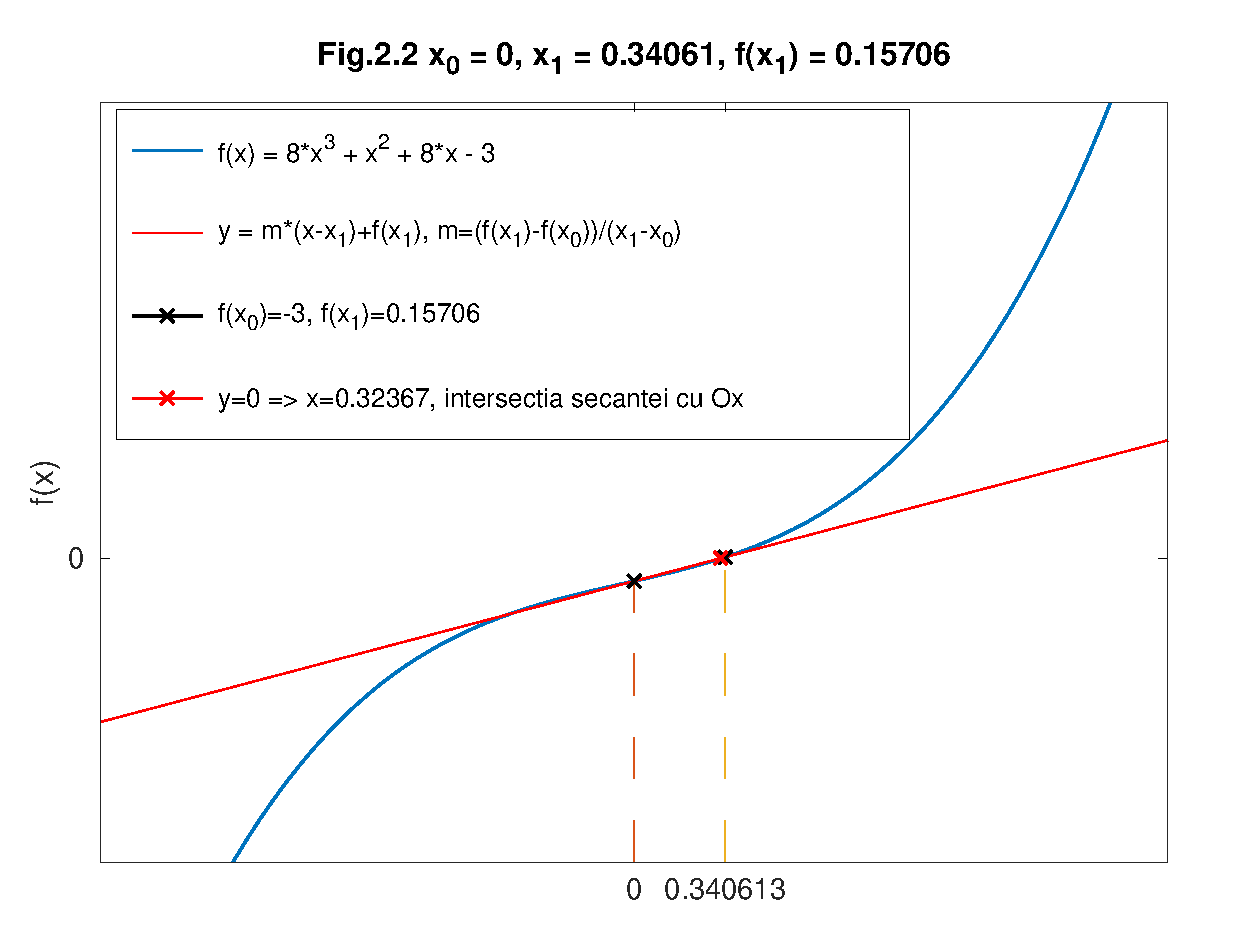
\includegraphics[height=90mm]{octave-fig/Fig.2.2.eps}
    \end{center}
\end{figure}
\begin{figure}[htbp]
    \begin{center}
        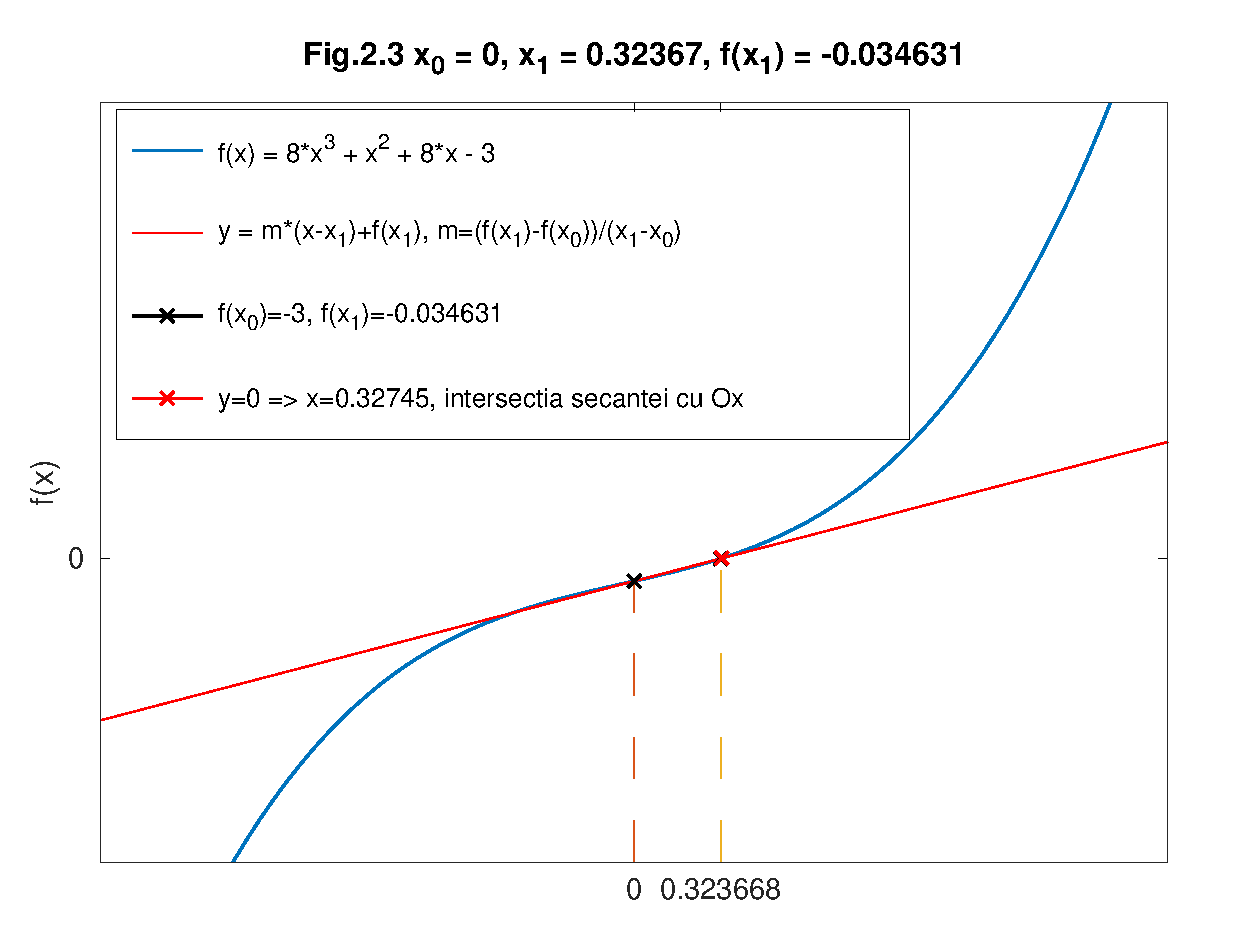
\includegraphics[height=90mm]{octave-fig/Fig.2.3.eps}
        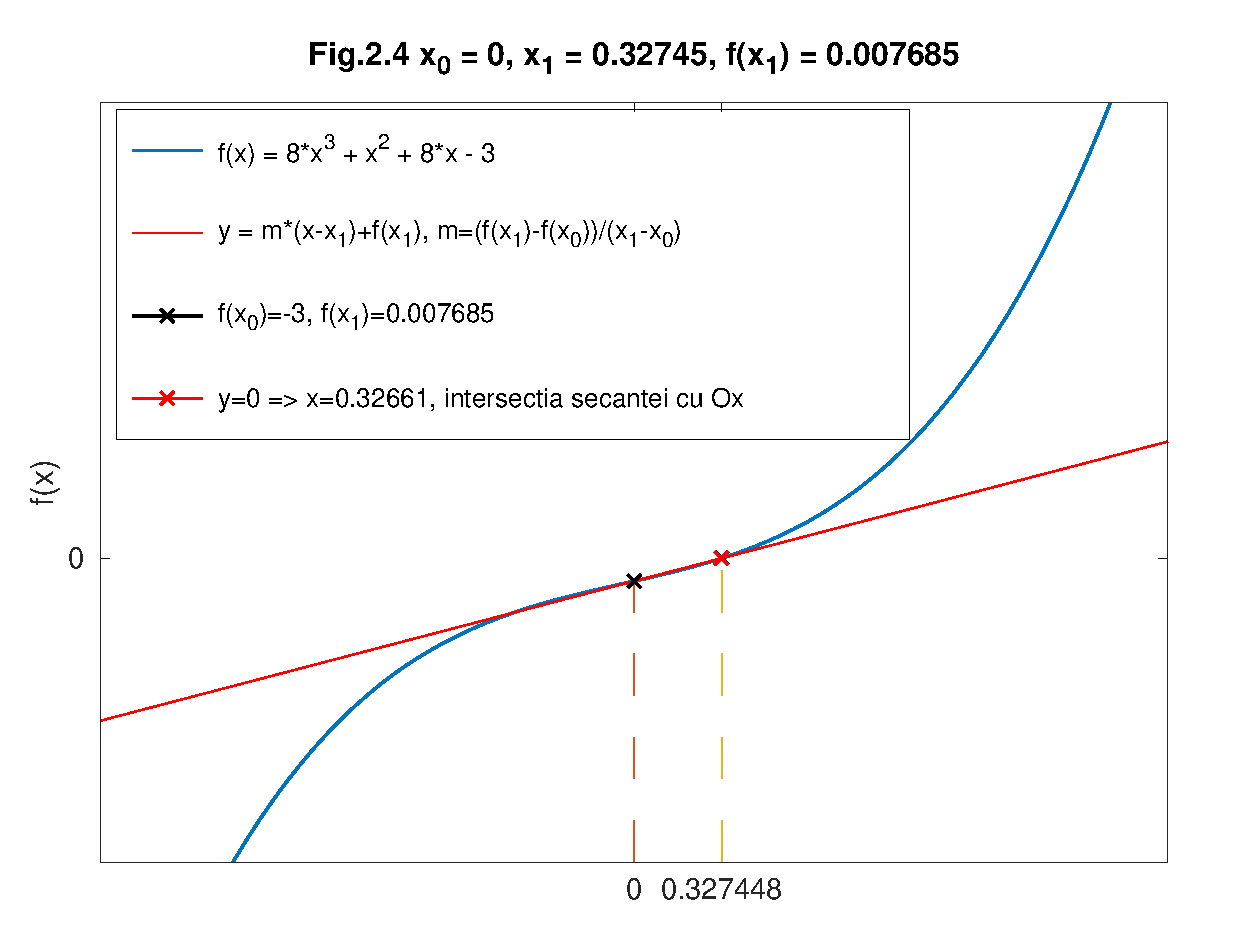
\includegraphics[height=90mm]{octave-fig/Fig.2.4.eps}
    \end{center}
\end{figure}
\newpage

(3) $f(x)=x^3-4x+2, f(x)=0, x=?$, prin metoda bisectiei, având $a=0, b=1, \varepsilon=0.01$.\\

\scriptsize
\begin{verbatim}
# Cod octave
f = @(x) x.^3-4*x+2;
a = 0;
b = 1;
epsilon = 0.01;
x_m = (a+b)/2;
i = 1;
max_i = 10;
while abs(f(x_m)) > epsilon 
    if max_i < i
        printf("Solution not found!\n");
        break;
    endif

    printf("i=%d & a=%f & b=%f & x_m=%f & f(x_m)=%f\n",i,a,b,x_m,f(x_m));
    print_graph(f, a, b, i);
    x_m = (a+b)/2;
    if f(x_m)*a < 0
        b = x_m;
    else
        a = x_m;
    endif
    i++;
endwhile
\end{verbatim}
\normalsize
$f(a)*f(b)<0 => Solutia \in [a,b]$\\\\
\begin{tabular}{ c | c | c | c | c }
    i=1 & a=0.000000 & b=1.000000 & x_m=0.500000 & f(x_m)=0.125000\\\hline
    i=2 & a=0.500000 & b=1.000000 & x_m=0.500000 & f(x_m)=0.125000\\\hline
    i=3 & a=0.500000 & b=0.750000 & x_m=0.750000 & f(x_m)=-0.578125\\\hline
    i=4 & a=0.500000 & b=0.625000 & x_m=0.625000 & f(x_m)=-0.255859\\\hline
    i=5 & a=0.500000 & b=0.562500 & x_m=0.562500 & f(x_m)=-0.072021\\\hline
    i=6 & a=0.531250 & b=0.562500 & x_m=0.531250 & f(x_m)=0.024933\\\hline
    i=7 & a=0.531250 & b=0.546875 & x_m=0.546875 & f(x_m)=-0.023945\\\hline
    i=8 & a=0.539062 & b=0.546875 & x_m=0.539062 & f(x_m)=0.000395\\
\end{tabular}
\\\\$Solutia=x_m=0.539062$

\begin{figure}[htbp]
    \begin{center}
        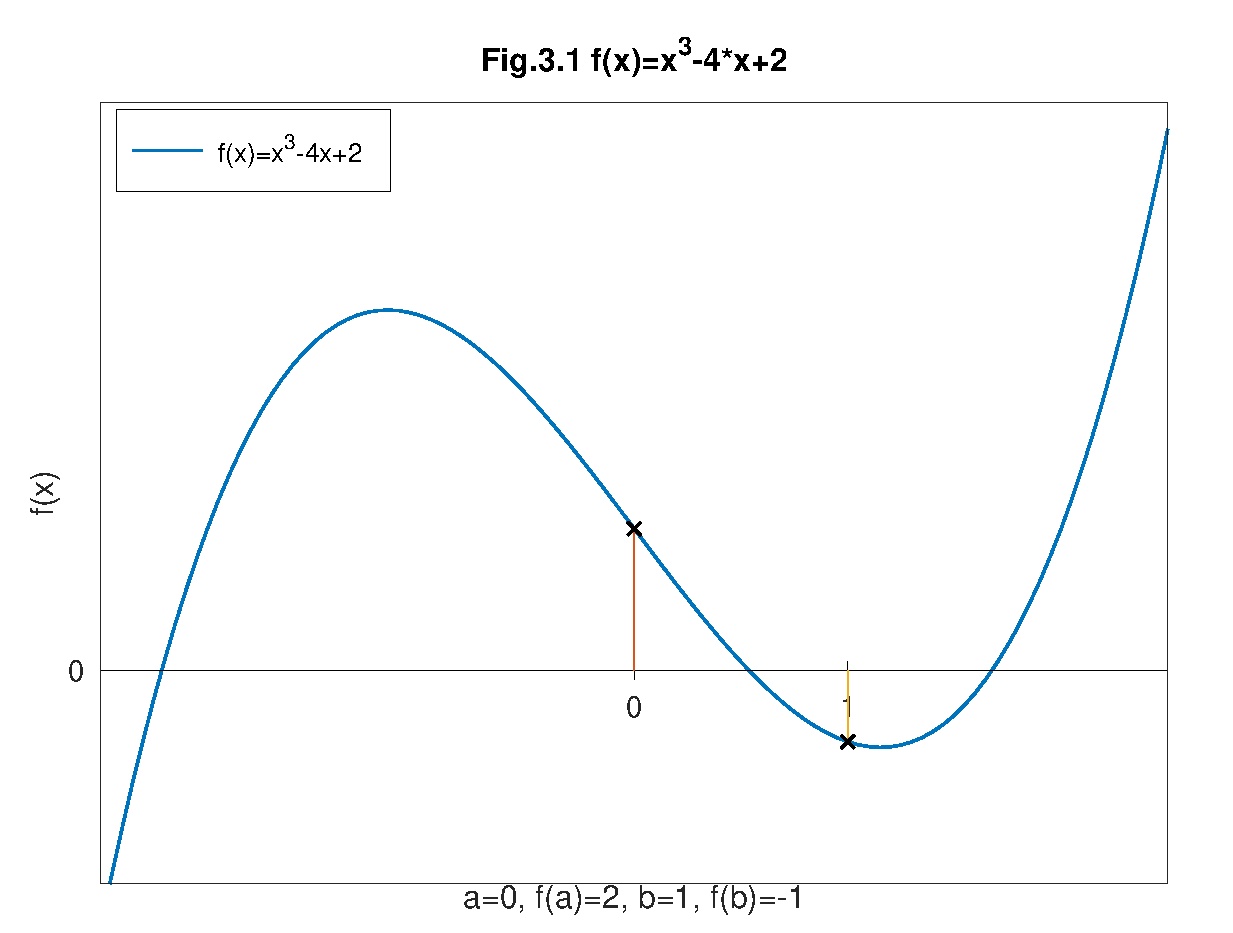
\includegraphics[height=90mm]{octave-fig/Fig.3.1.eps}
        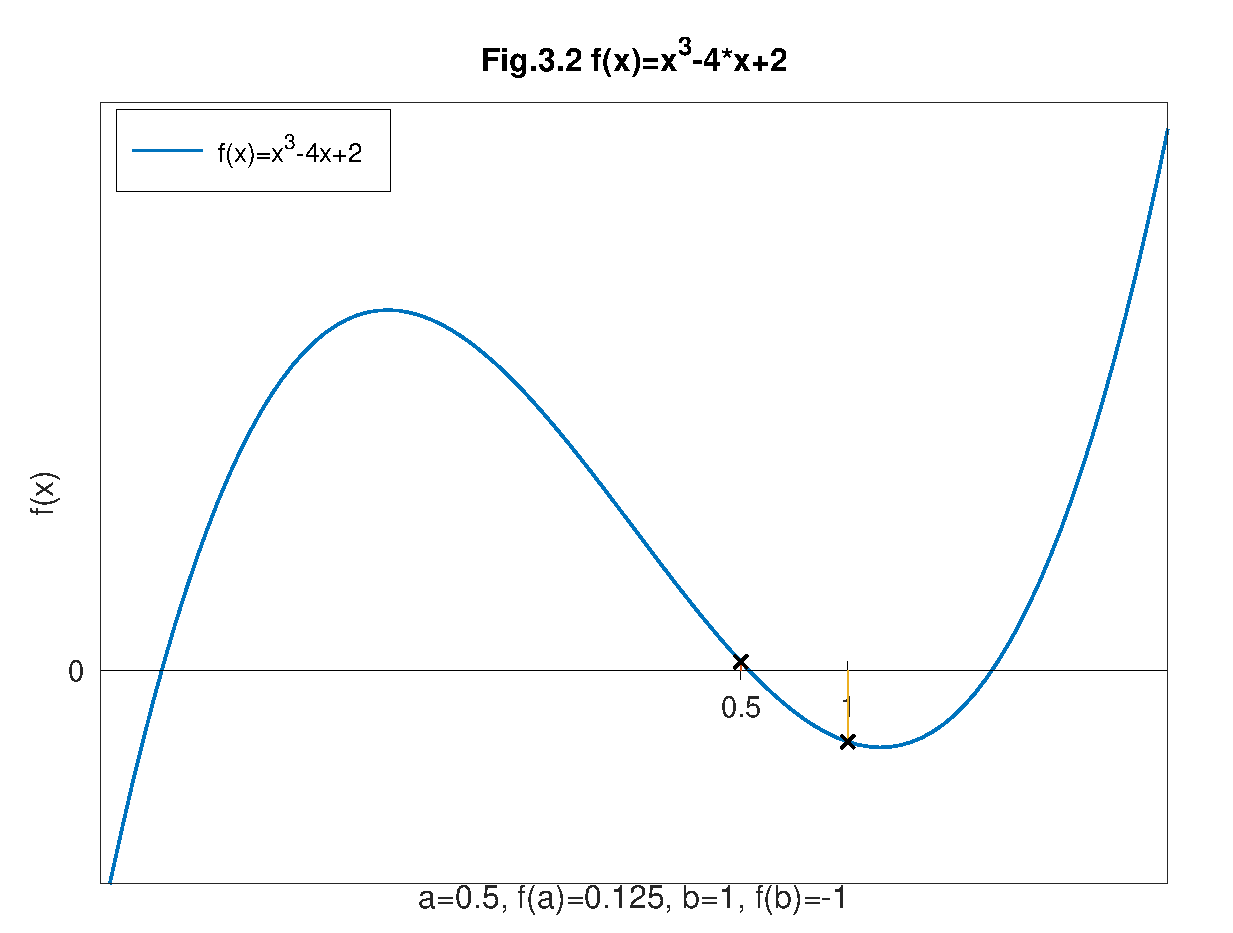
\includegraphics[height=90mm]{octave-fig/Fig.3.2.eps}
    \end{center}
\end{figure}
\begin{figure}[htbp]
    \begin{center}
        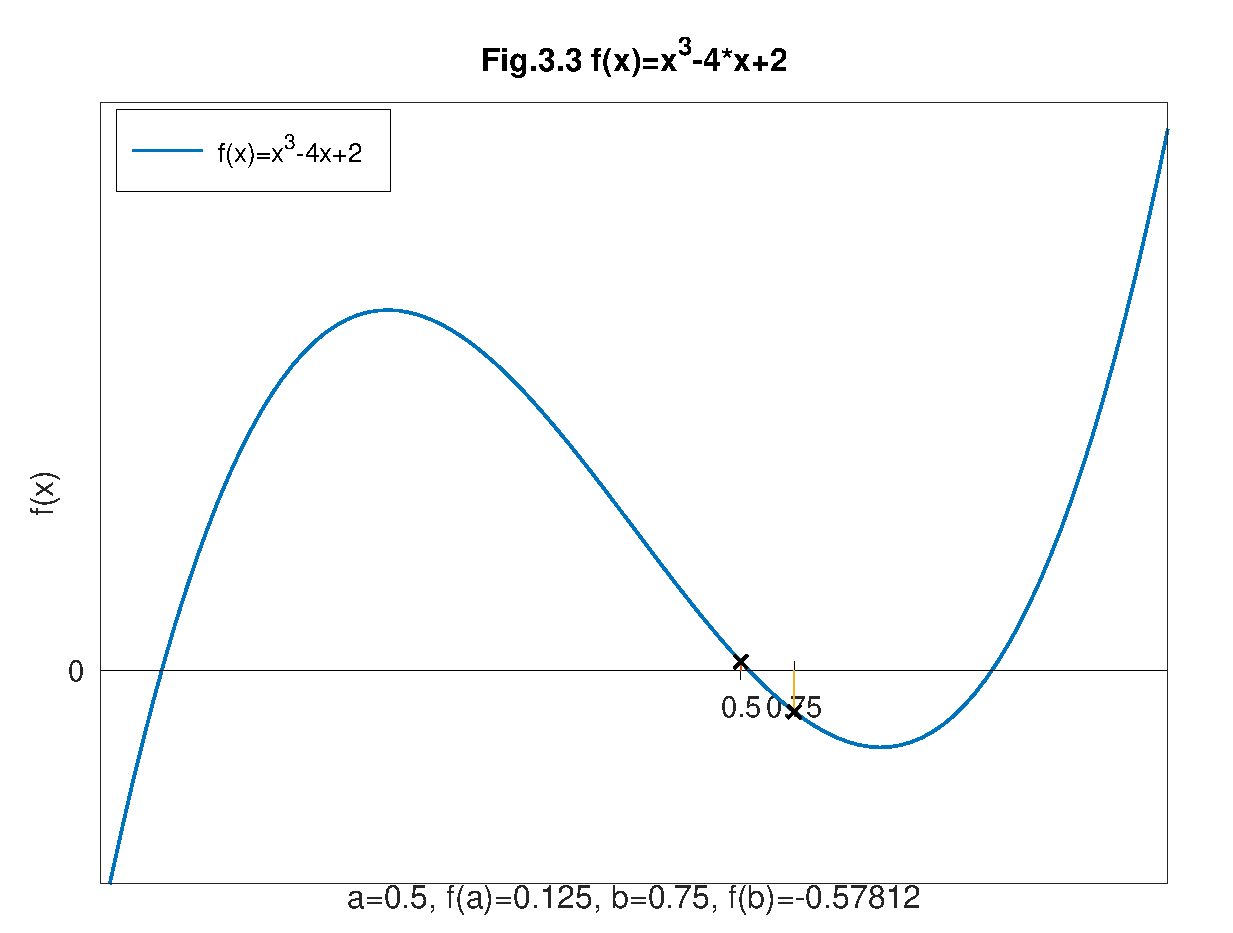
\includegraphics[height=90mm]{octave-fig/Fig.3.3.eps}
        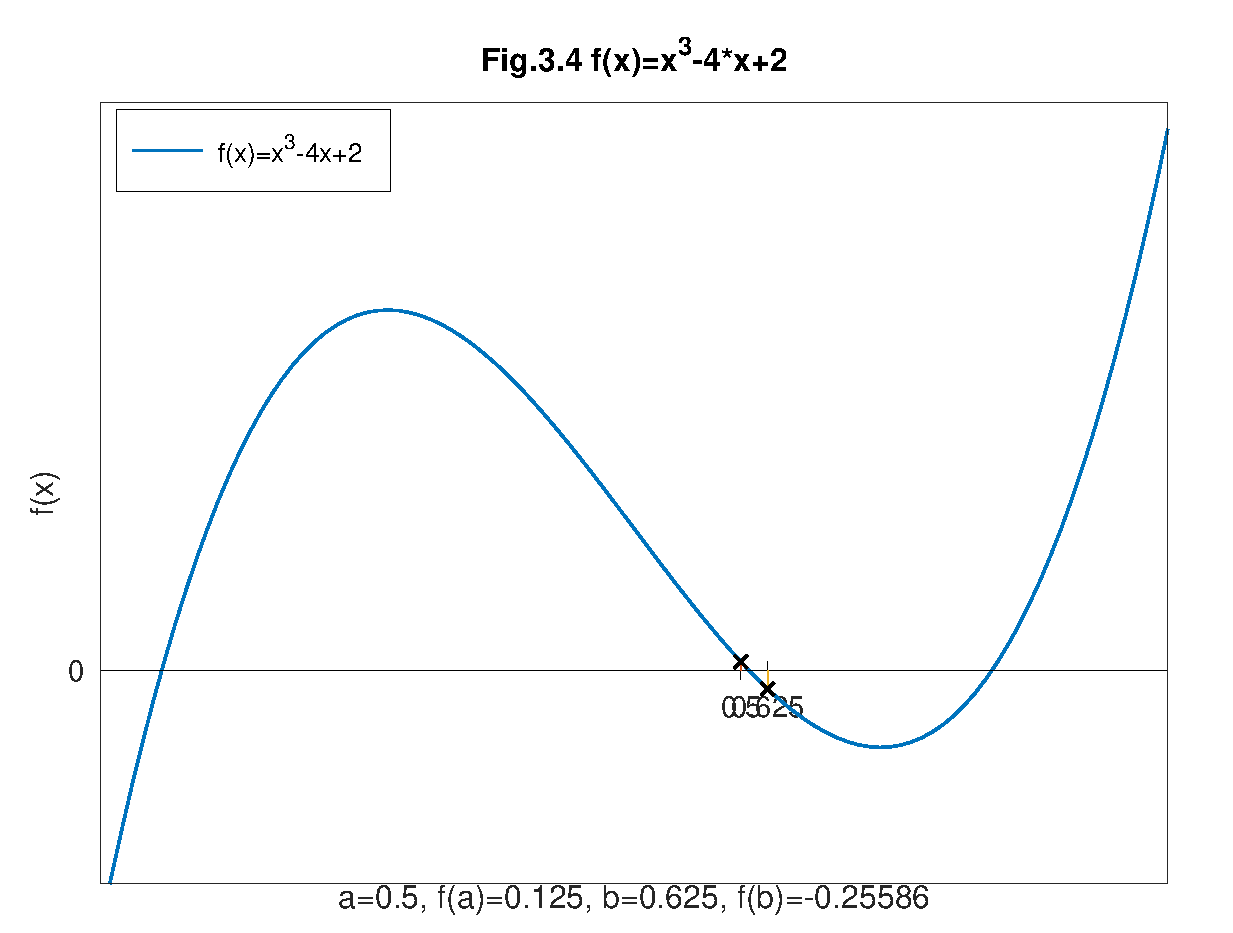
\includegraphics[height=90mm]{octave-fig/Fig.3.4.eps}
    \end{center}
\end{figure}
\begin{figure}[htbp]
    \begin{center}
        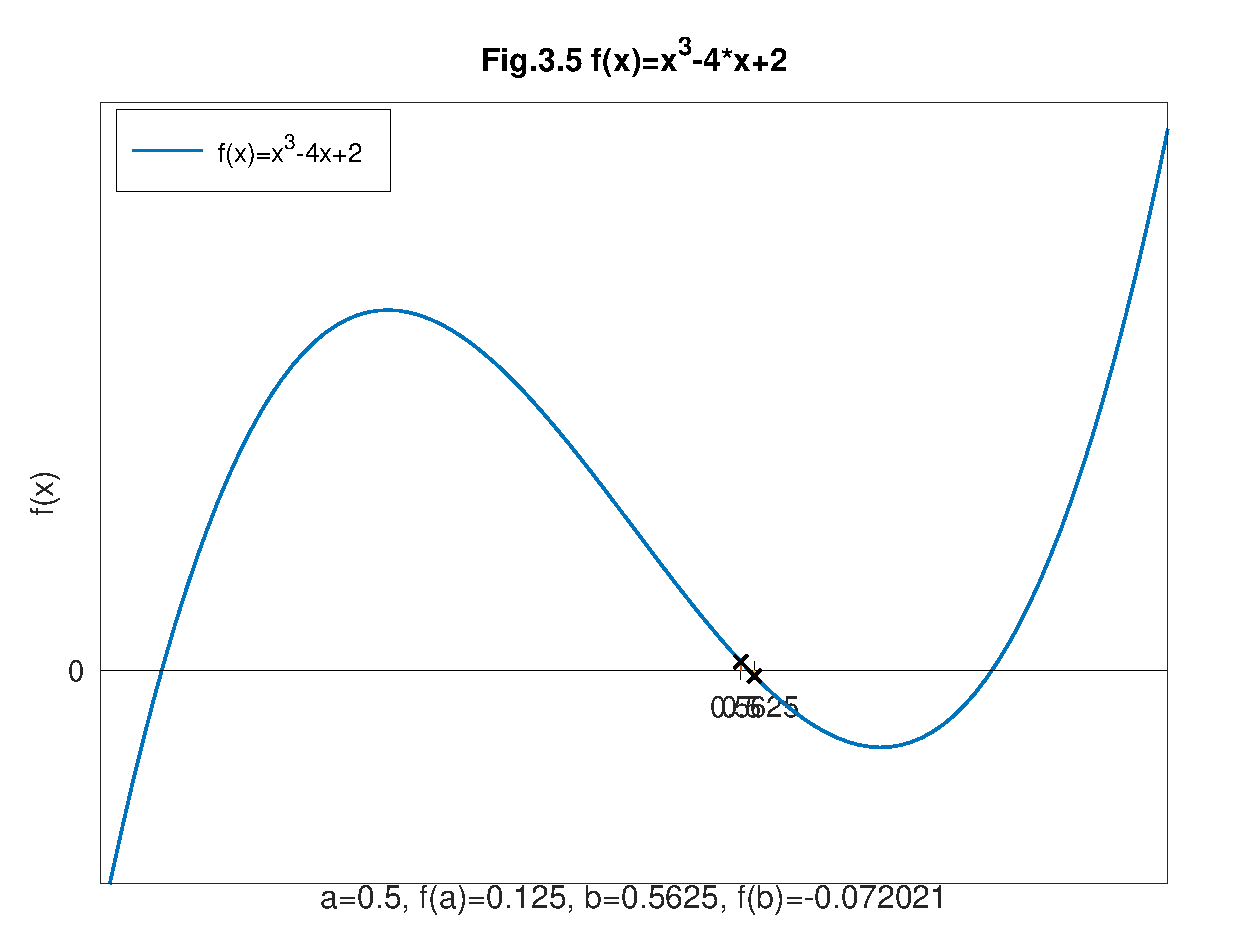
\includegraphics[height=90mm]{octave-fig/Fig.3.5.eps}
        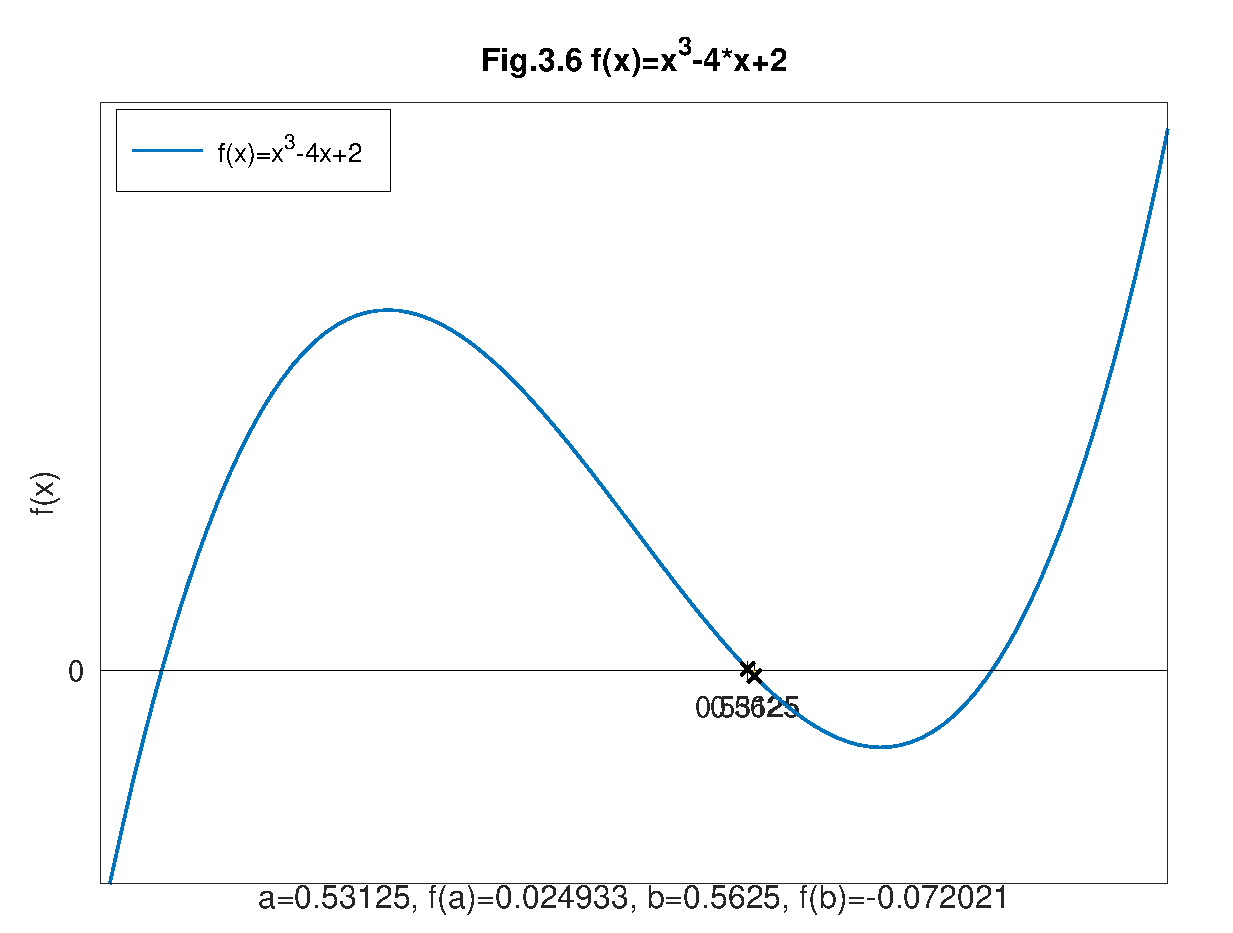
\includegraphics[height=90mm]{octave-fig/Fig.3.6.eps}
    \end{center}
\end{figure}
\begin{figure}[htbp]
    \begin{center}
        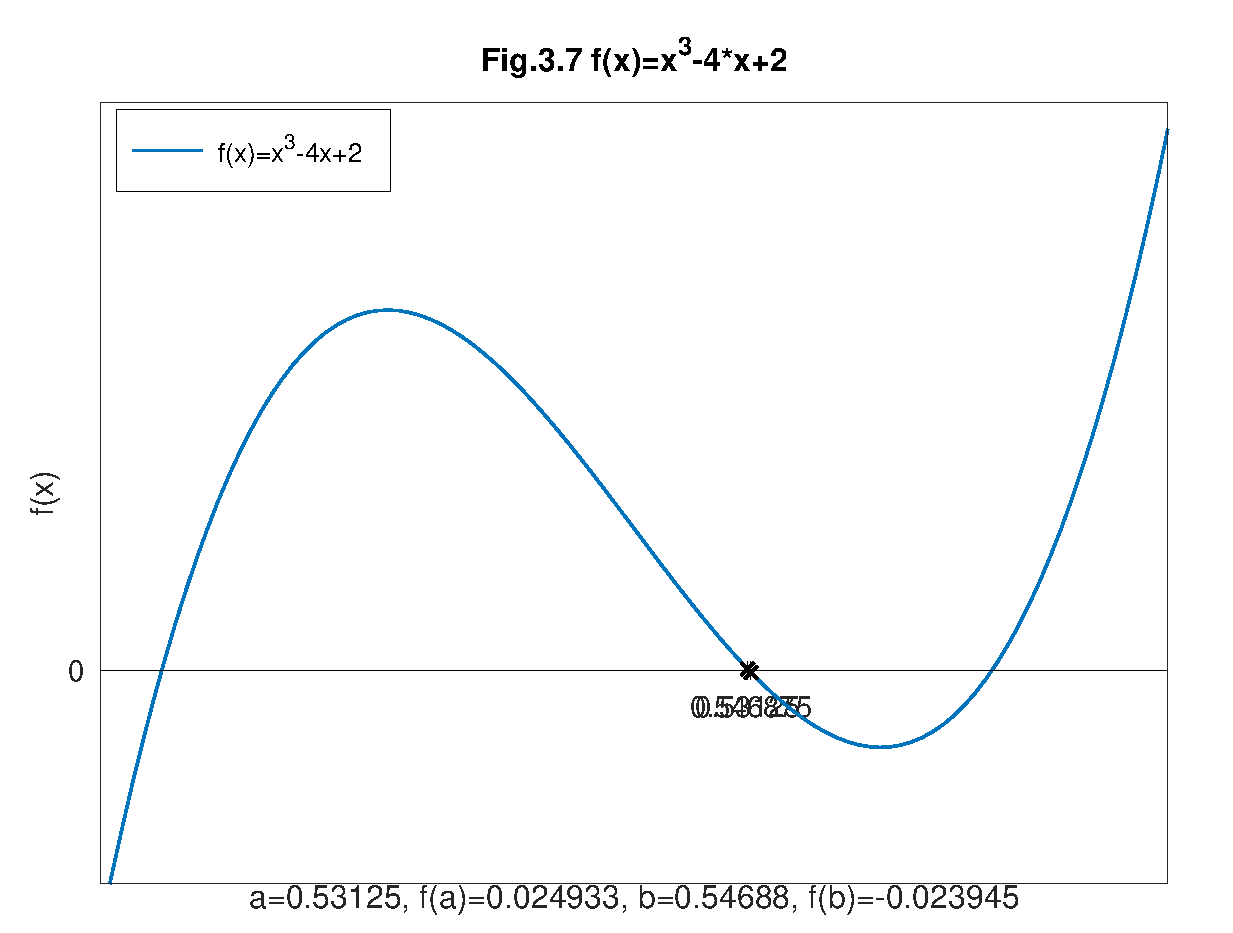
\includegraphics[height=90mm]{octave-fig/Fig.3.7.eps}
        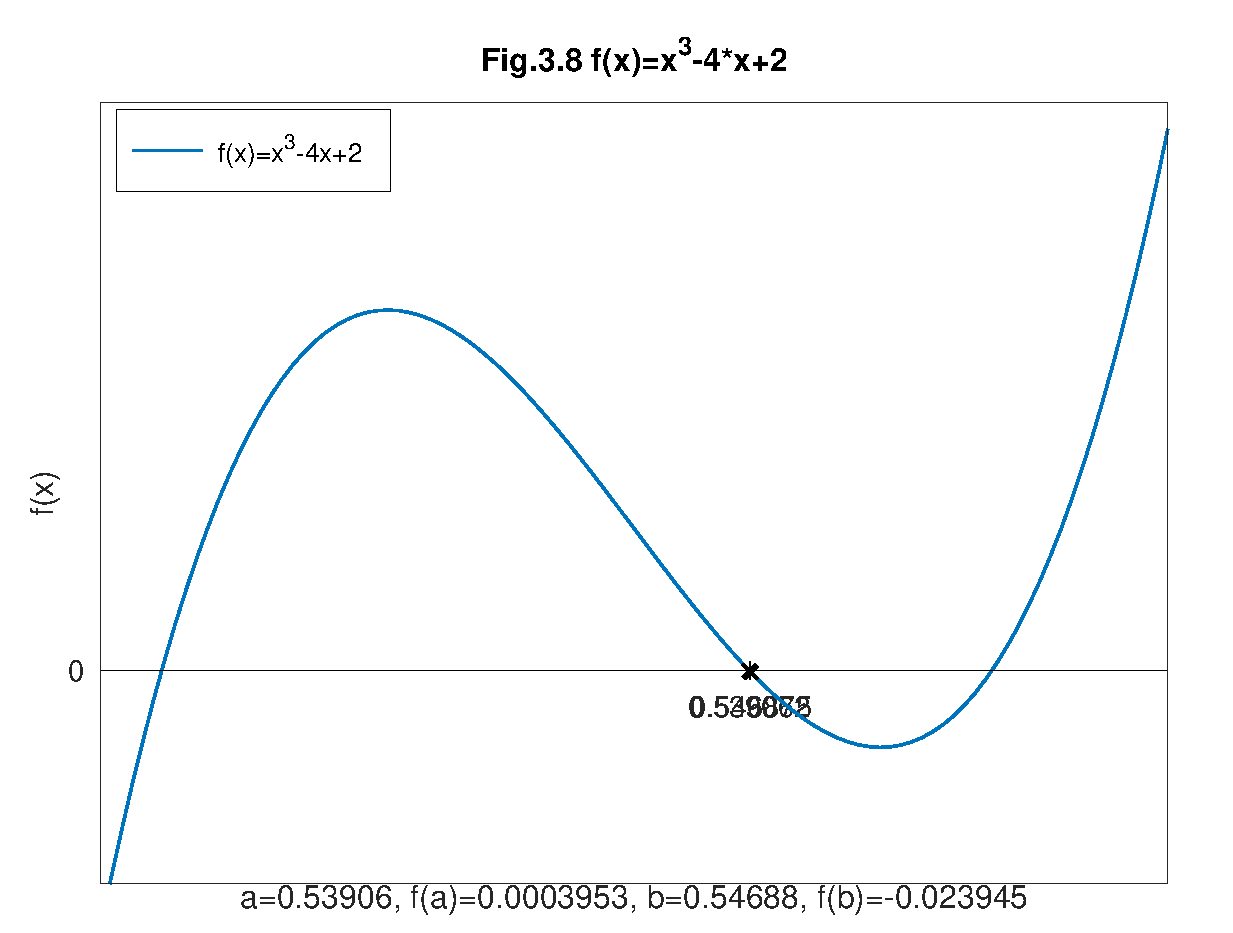
\includegraphics[height=90mm]{octave-fig/Fig.3.8.eps}
    \end{center}
\end{figure}
\newpage

(4) $f(x)=x^3-4x+2, x_1=1, x_2= ?$ prin metoda lui Newton-Raphson.\\

Punctul $(x_2,0)$ reprezintă intersecția cu $Ox$ a tangentei prin $(x_1,f(x_1))$.
Panta acestei tangente este dată de derivata funcției $f$ pentru $x_1=1$.
$m=f'(x_1)$. De asemenea aceasta pantă se poate calcula din ecuația tangentei,
pentru $m=\frac{f(x_1)-y}{x_1-x_2}, y=0$.\\
Din $m=f'(x_1), m=\frac{f(x1)}{x_1-x_2} => f'(x_1)=\frac{f(x_1)}{x_1-x_2}$.\\
Calculând pentru $x_2$, avem $x_2=x_1-\frac{f(x_1)}{f'(x_1)}=0$.
\begin{figure}[htbp]
    \begin{center}
        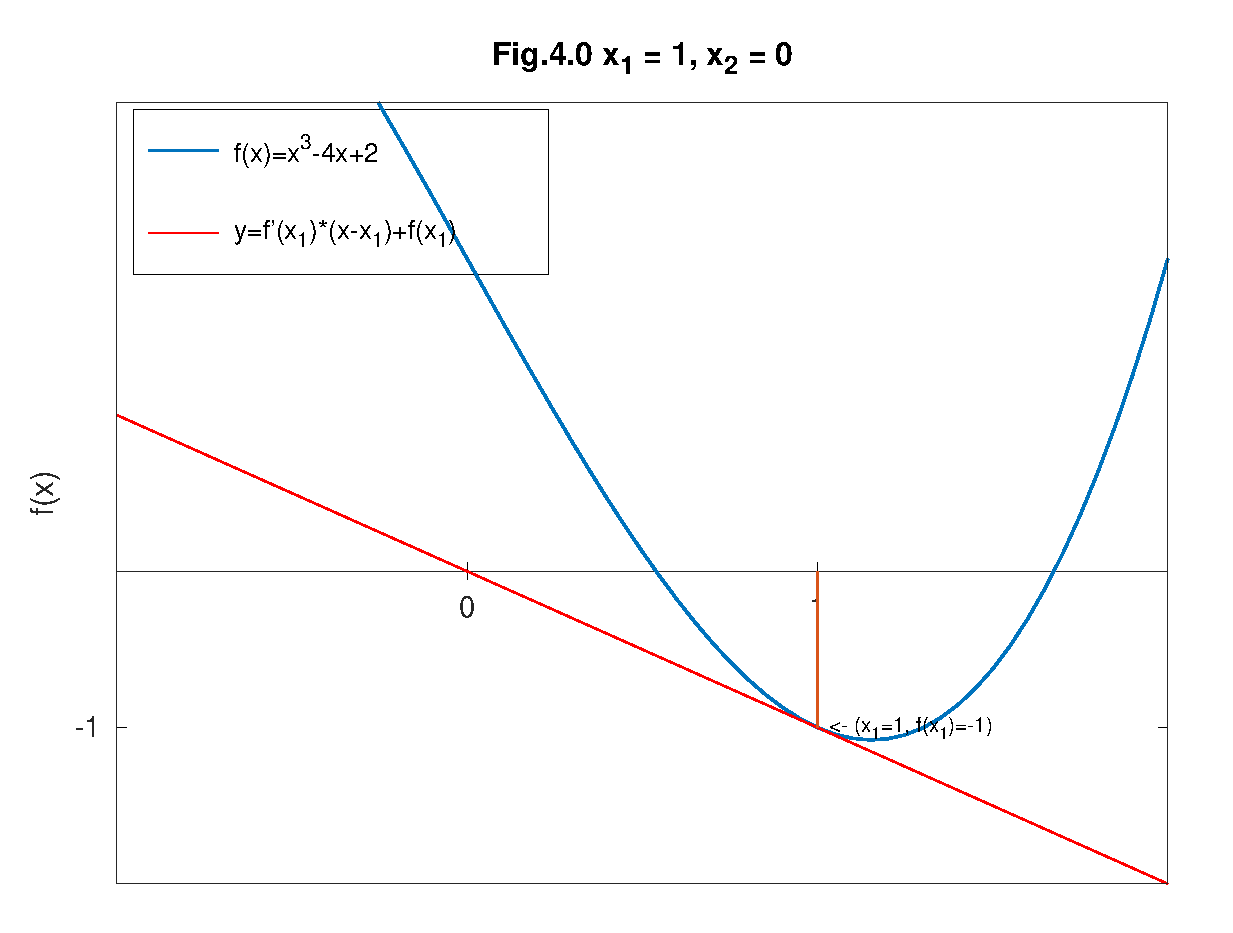
\includegraphics[height=90mm]{octave-fig/Fig.4.0.eps}
    \end{center}
\end{figure}
\begin{verbatim}
    # Cod octave
    f = @(x) x.^3 - 4*x + 2;
    df = @(x) 3*x^2 - 4;
    x_1 = 1;
    x_2 = x_1 - f(x_1)/df(x_1);
\end{verbatim}
\newpage

(5) $f(x)=x^3-4x+2$ Daca $x_0=0$ si $x_1=1$, cat sunt $x_2$ si $x_3$ din metoda secantei?\\
Definim relația $y$ în funcție de $x$ ca fiind secanta care trece prin punctele $(x_0, f(x_0)), (x_1, f(x_1))$.

Panta calculată cu aceste puncte este: $m=\frac{f(x_1)-f(x_0)}{x_1-x_0}$.

Panta calculată cu punctul $(x_1, f(x_1))$ și alt punct al secantei este:
$m=\frac{f(x_1)-y}{x_1-x}$. 

Din
$m=\frac{f(x_1)-f(x_0)}{x_1-x_0}, m=\frac{f(x_1)-y}{x_1-x} =>\frac{f(x_1)-f(x_0)}{x_1-x_0} = \frac{f(x_1)-y}{x_1-x}$.

Izolându-l pe $x$ obținem:

$x_1-x = \frac{(f(x_1)-y)(x_1-x_0)}{f(x_1)-f(x_0)} <=>
x = x_1-\frac{(f(x_1)-y)(x_1-x_0)}{f(x_1)-f(x_0)}$.

Definim punctul $(x_2,0)$ ca fiind intersecția secantei cu $Ox$, deci $y=0$.

$y=0, x=x_2 => x_2 = x_1-\frac{f(x_1)(x_1-x_0)}{f(x1)-f(x_0)}$.

\scriptsize
\begin{verbatim}
# Cod octave
f = @(x) x^3 - 4*x + 2;
x_0 = 0;
x_1 = 1;
x_2 = x_1 - (f(x_1)*(x_1-x_0))/(f(x_1)-f(x_0));
x_3 = x_2 - (f(x_2)*(x_2-x_1))/(f(x_2-f(x_1)));
printf("$x_2=%.3f, x_3=%.3f$\n", x_2, x_3);
\end{verbatim}
\normalsize

Soluțiile calculate sunt: $x_2=0.667, x_3=4.000$.

\begin{figure}[htbp]
    \begin{center}
        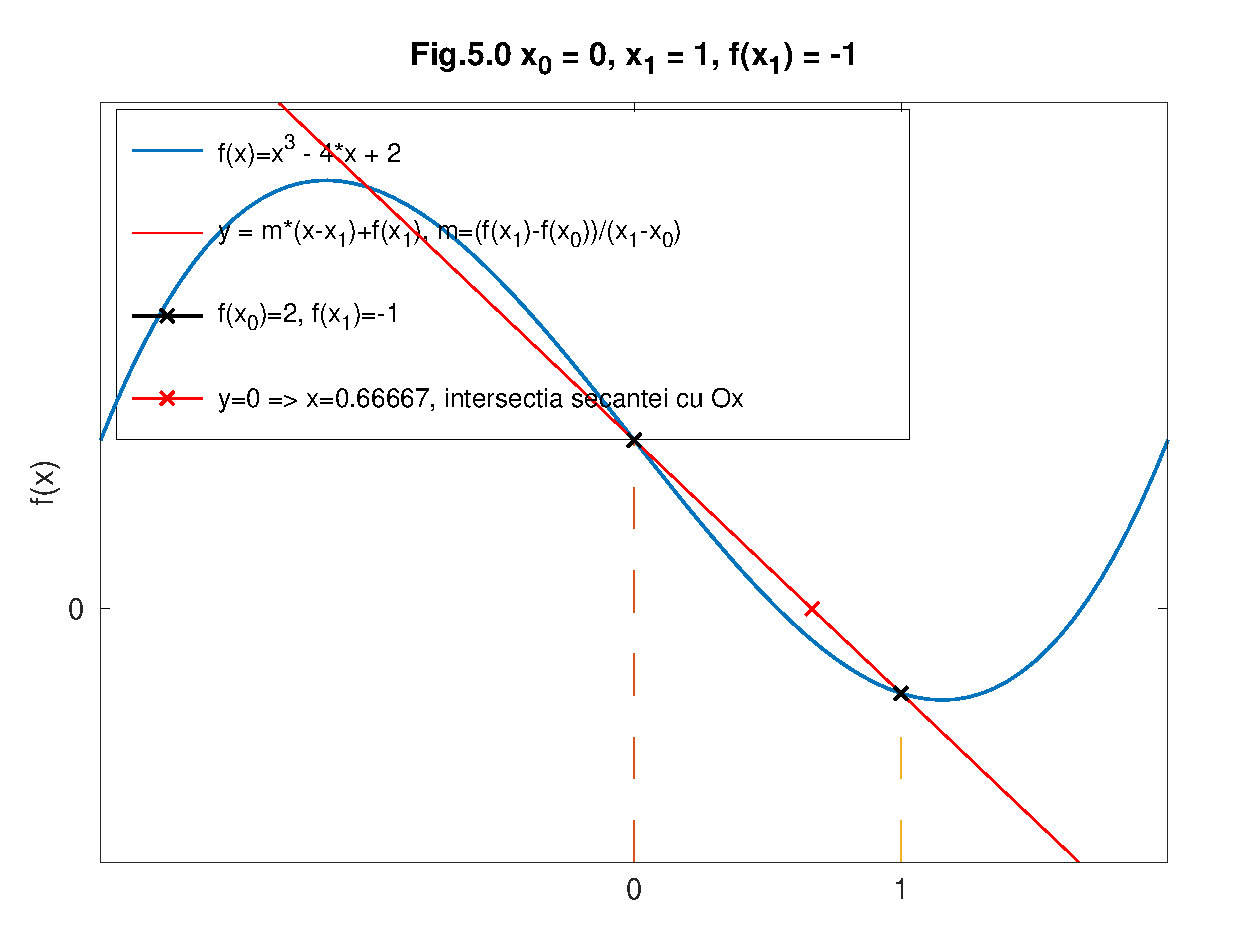
\includegraphics[height=70mm]{octave-fig/Fig.5.0.eps}
    \end{center}
\end{figure}

\end{document}